\subsubsection{Definición de entradas y salidas de las redes neuronales}\label{inputs-outputs}

Antes de continuar explicando los pasos llevados a cabo, se tiene que definir la estructura del \textit{dataset} que se necesita para entrenar a las redes neuronales. Uno de los principales requisitos en el diseño de redes neuronales es la correcta especificación del vector de entrada y salida de la red neuronal. La cantidad de variables y el tipo de variables que se usarán en la red es una de las principales claves para que el modelo funcione de forma satisfactoria. En este apartado se explicará tanto la estructura del vector de entrada como la estructura del vector de salida acompañado de ejemplos gráficos.
\newline

Los modelos con los que se trabaja tendrán en el vector de entrada valores que representan la fecha y la hora representados con los siguientes atributos: \textit{hour} ($h$), \textit{day\_of\_week}($d$) y \textit{month}($m$). Para ello es necesario que los viajes se agrupen por intervalos, creando de este modo nuevas columnas(\textit{quantity\_$j$}), siendo $j$ un entero que represente al identificador de la estación dentro de la red. Estas columnas serán referenciadas con una $q$. En total hay $633$ estaciones en la ciudad de Chicago. Por lo que para cada intervalo, la red neuronal contará con $636$ valores de entrada. Se pueden ver ejemplos gráficos en la Figura \ref{fig:models-design-1} y \ref{fig:models-design-2}. El tamaño del \textit{dataset} final será de \small\verb|n_intervals| $\times ($ \small\verb|n_stations| $+ 3)$.
\newline

Lo más básico sería crear un modelo que toma como entrada un único intervalo y predijese un único intervalo representado por el vector de salida. Para este modelo, la entrada de la red sería de $636$, formado por $[h, d, m, q_j], j$ $ \forall$ $[1, 633]$, donde $h$, $d$ y $m$ son las tres variables que aportan información sobre el intervalo y \textit{$q_j, j\in [1, 633]$} son valores que representan la cantidad de viajes iniciados para la estación $j$ en dicho intervalo. La salida sería un vector de $633$ elementos que representaría la predicción del intervalo inmediatamente posterior al intervalo de entrada y tendría el mismo orden que el vector de entrada \textit{quantity\_$j, j\in [1, 633]$}.
\newline

Si se quiere usar más intervalos en el modelo, el vector de entrada tendrá un número de elementos múltiplo de $636$. Por ejemplo, si se quieren usar 5 intervalos como vector de entrada, entonces la red tendrá una primera capa con $636 \times 5 = 3180$ unidades o neuronas. De forma similar, si se quiere que la salida de la red sea un vector que contenga la predicción para todas las estaciones de la red, el tamaño del vector resultante será múltiplo de $633$. 
\newline

En los modelos \acrfull{ar}, a pesar de ser modelos capaces de predecir múltiples intervalos si fuese necesario, la salida de estos modelos siempre serán de un intervalo. Esto es debido a que es necesario calcular todos los intervalos de forma independiente pues el modelo \acrshort{ar} usa su propia predicción como vector de entrada. Se puede ver más información sobre esto en la Sección \ref{window_ar} y \ref{model_ar}.
\newline

A continuación, se pueden ver gráficamente varios ejemplos de distintas configuraciones de red usando diferentes combinaciones para la cantidad de intervalos de entrada y salida:


\begin{figure}[H]
    \centering
    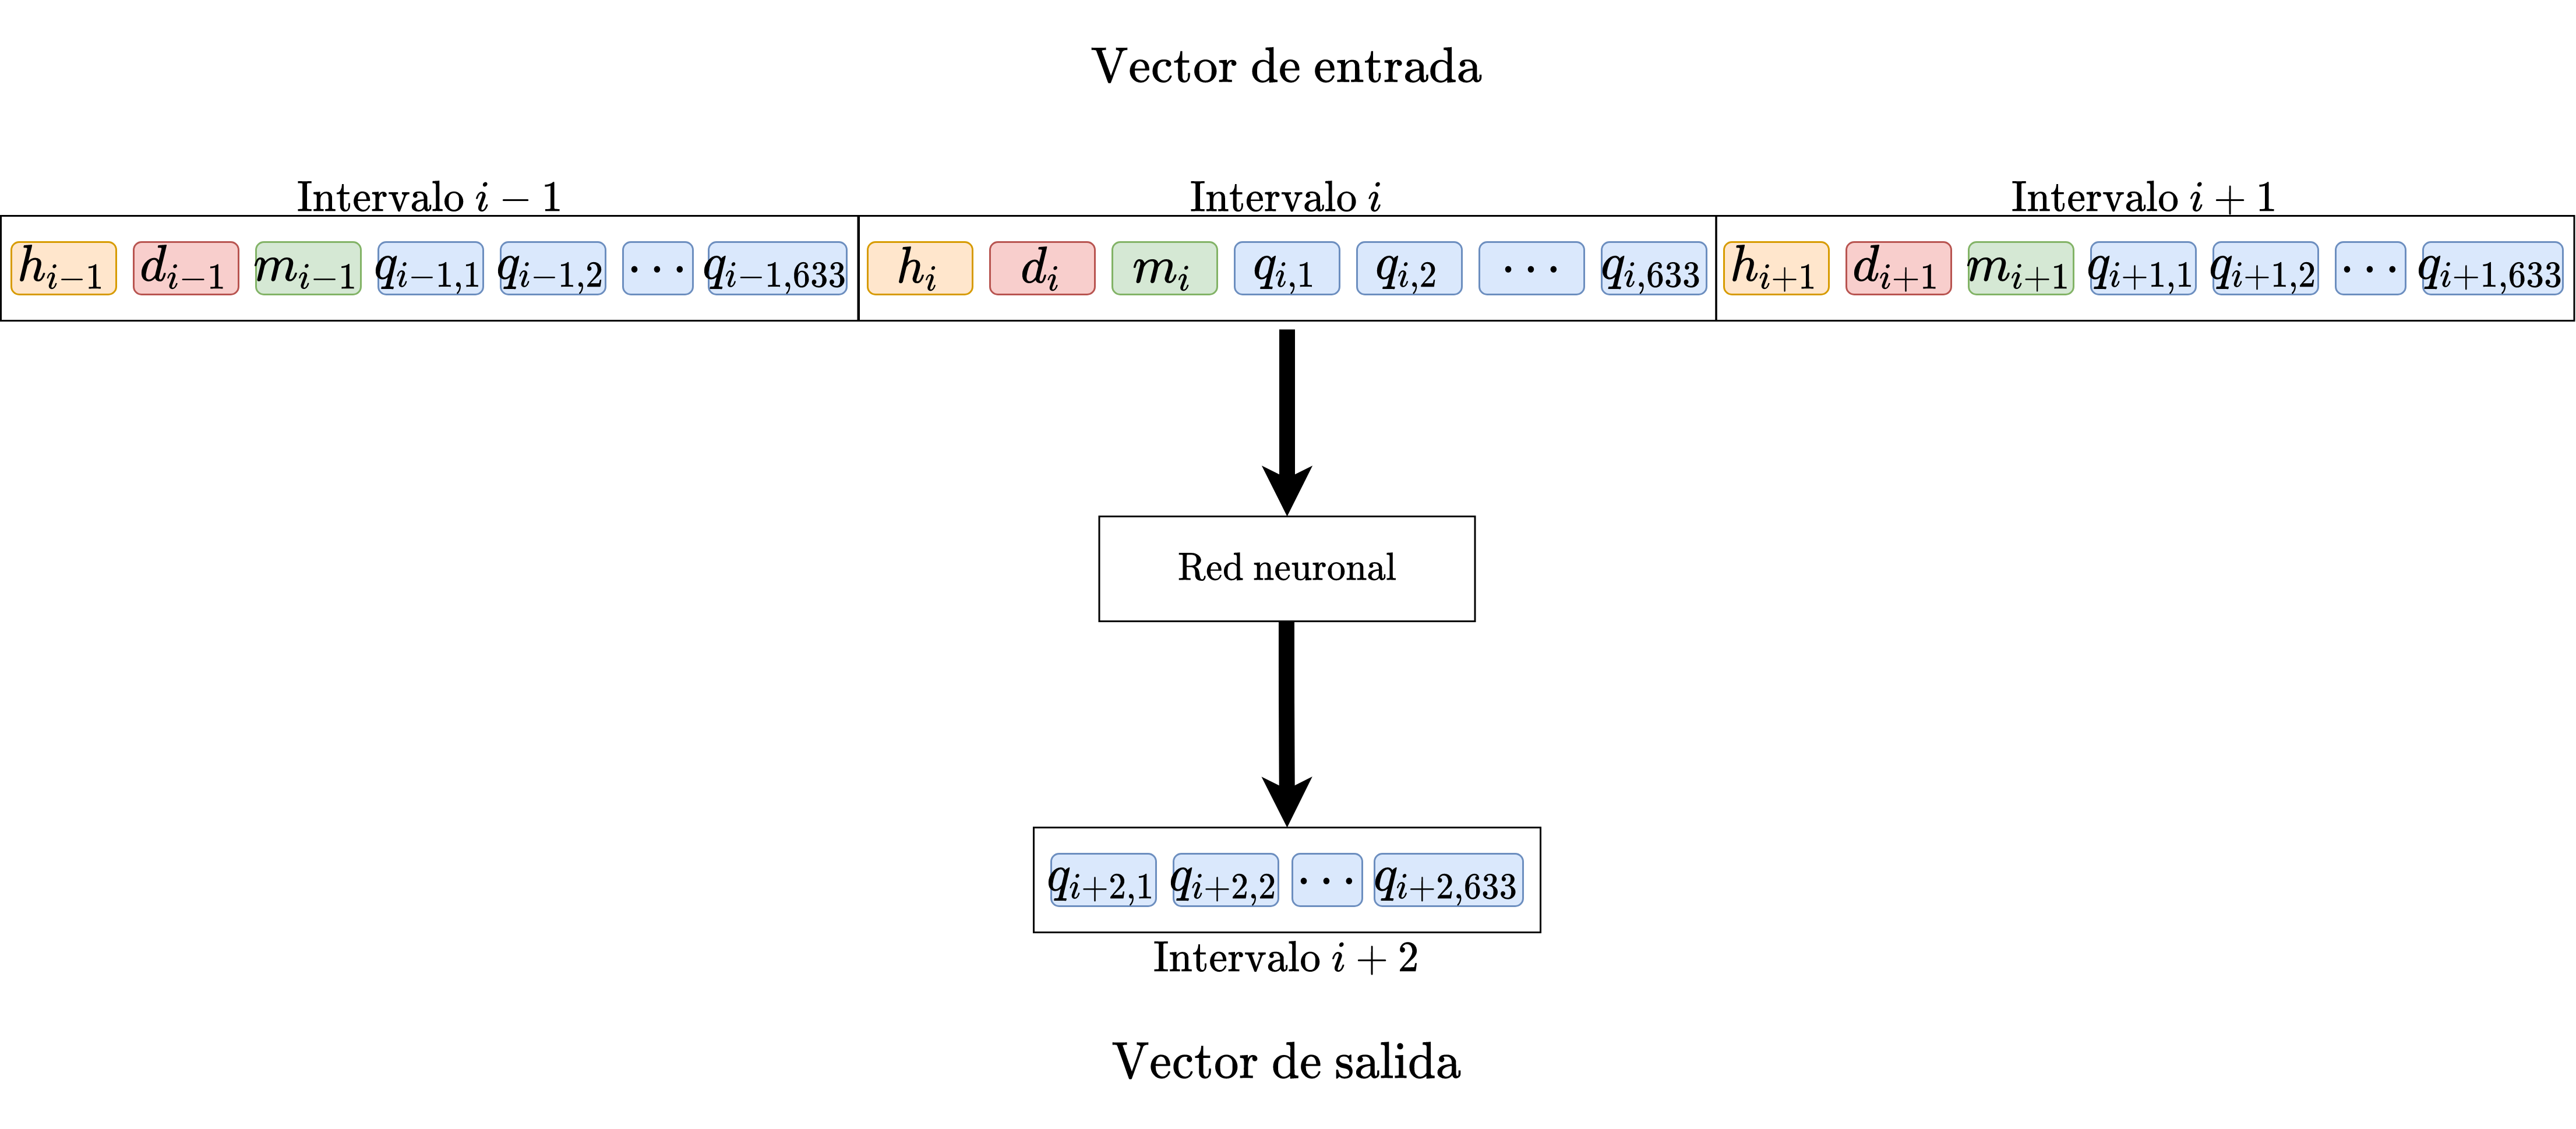
\includegraphics[width=14cm]{images/solution/preprocessing/models-design-1.png}
    \caption{Ejemplo de red neuronal que usa 3 intervalos de entrada y predice 1 intervalo}
    \label{fig:models-design-1}
\end{figure}

\begin{figure}[H]
    \centering
    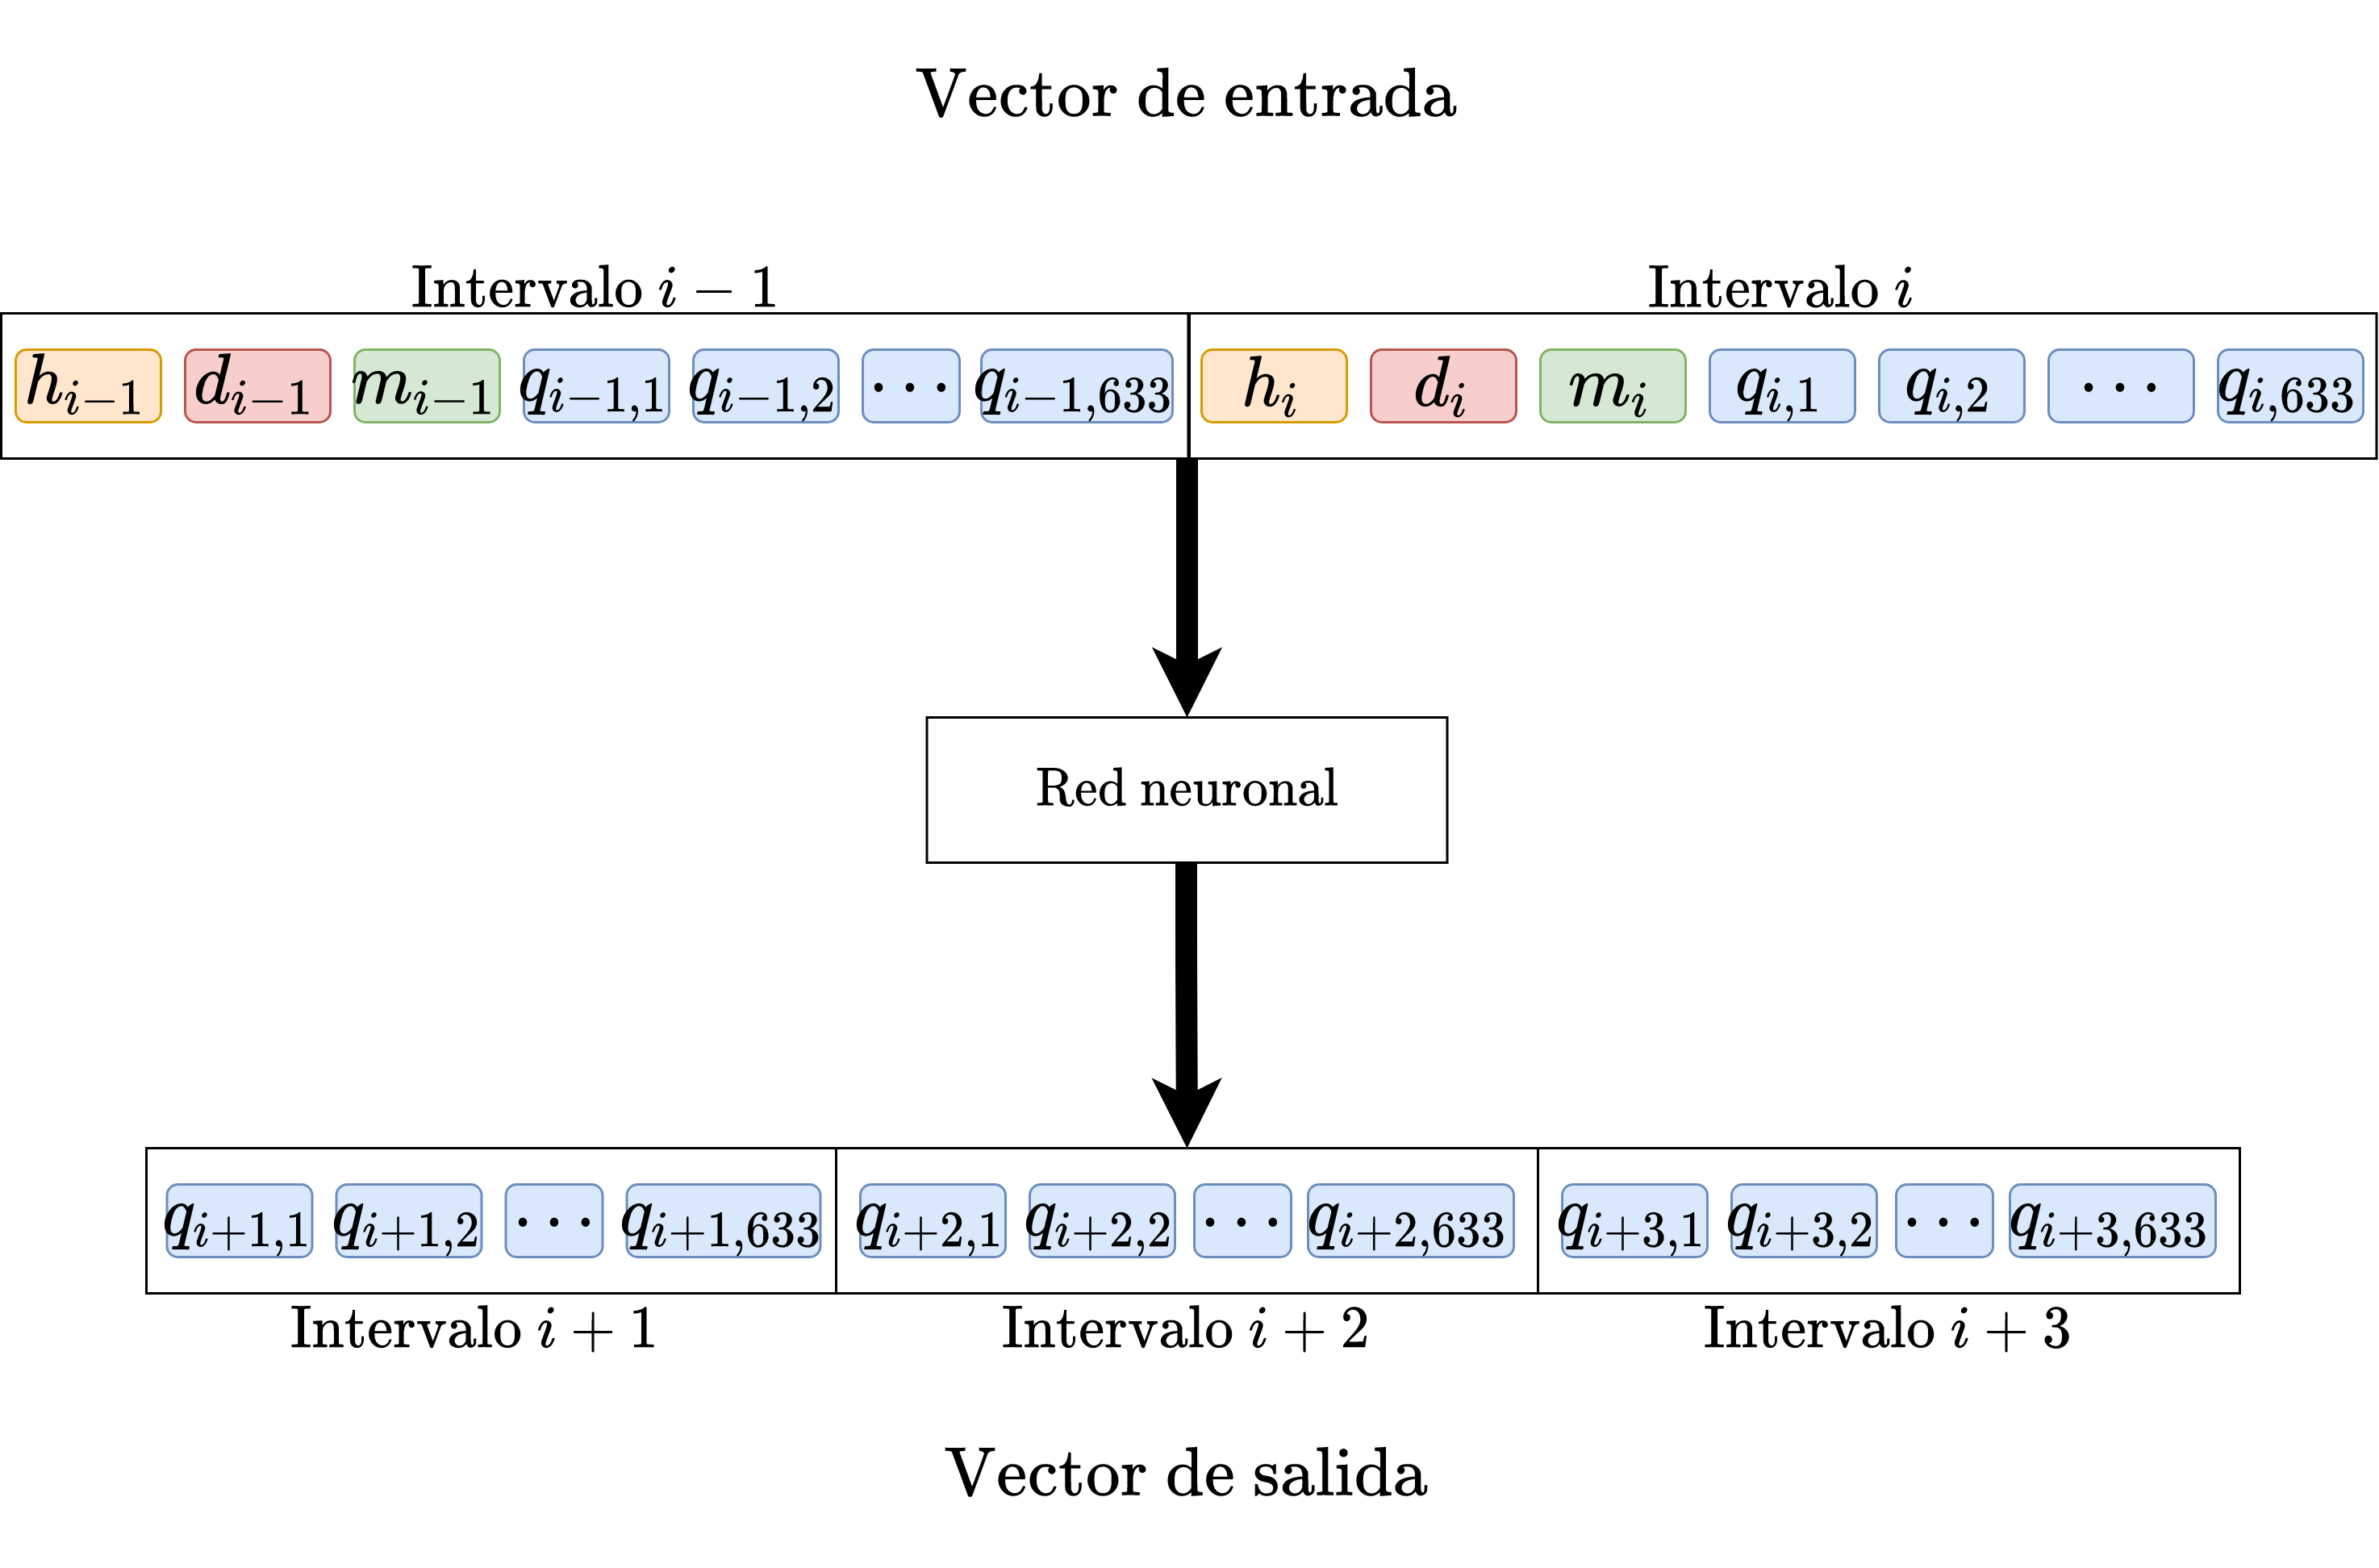
\includegraphics[width=14cm]{images/solution/preprocessing/models-design-2.png}
    \caption{Ejemplo de red neuronal que usa 2 intervalos de entrada y predice 3 intervalos}
        \label{fig:models-design-2}
\end{figure}


Esta forma de estructurar los datos y los modelos es muy flexible. Permite que el código se pueda adaptar fácilmente a otros \textit{datasets} y no sea único para la ciudad de Chicago. Además, también permite que se pueda trabajar con un grupo de estaciones más pequeño si se quisiese. Al ser cada columna una estación, simplemente filtrando por las columnas que sean de interés, se podría entrenar los modelos con dichas columnas. También cabría la posibilidad de trabajar por comunidades, agrupando las estaciones en función de una serie de reglas y poder de esa forma estudiar los patrones de un barrio y no de cada estación de forma particular como se realiza en este trabajo.
\newline